\documentclass[10pt,a4paper]{article}
\usepackage[utf8]{inputenc}
\usepackage[english]{babel}
\usepackage{amsmath}
\usepackage{amsfonts}
\usepackage{amssymb}
\usepackage{graphicx}
\usepackage{hyperref}
\usepackage{float}
\author{Anders Bo Justesen, \texttt{justesen@phys.au.dk}}
\title{\vspace{-3cm} Delphini-1 Project:\\Satellite Tracking Applications}
\date{\today}
\begin{document}
\maketitle

\section{Introduction}
I have developed two satellite tracking applications for the control room. The first application, \textit{Satellite Earth View} (\texttt{SEV}) displays a view of Earth from the satellite's position in orbit. The second application, \textit{Satellite Map View} (\texttt{SMV}) displays the satellite's current position on an interactive map. The front end of the applications are based on Google's mapping platform. This is done to ensure maximum compatibility, flexibility and extendability. The back end (the computation of the satellite's position) is written in Python and compiled in a module called \texttt{sattrack}.

\begin{figure}
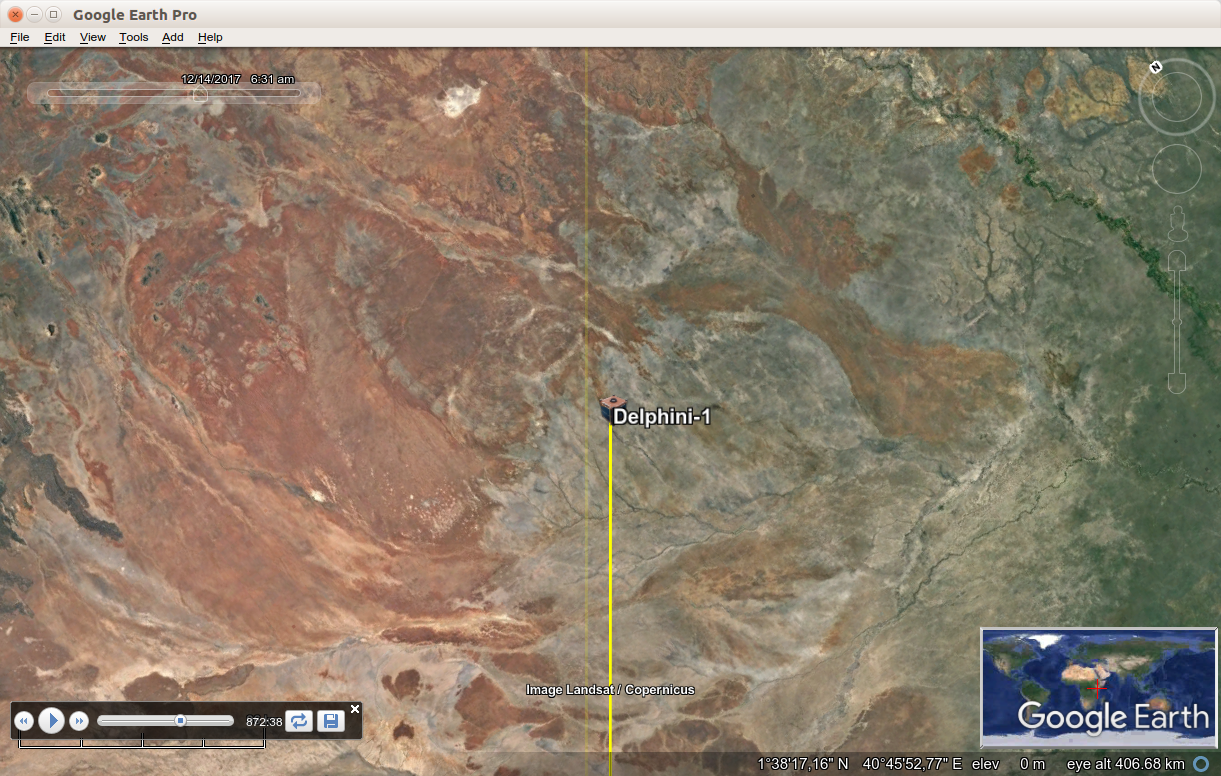
\includegraphics[width=\textwidth]{../Playing.png}
\caption{\texttt{SEV} showing the view of Earth underneath the ISS on 14/12 2017 6:31 UTC. It is possible to remove the satellite icon and orbit for a cleaner look.}
\label{Fig:SEV}
\end{figure}

\begin{figure}
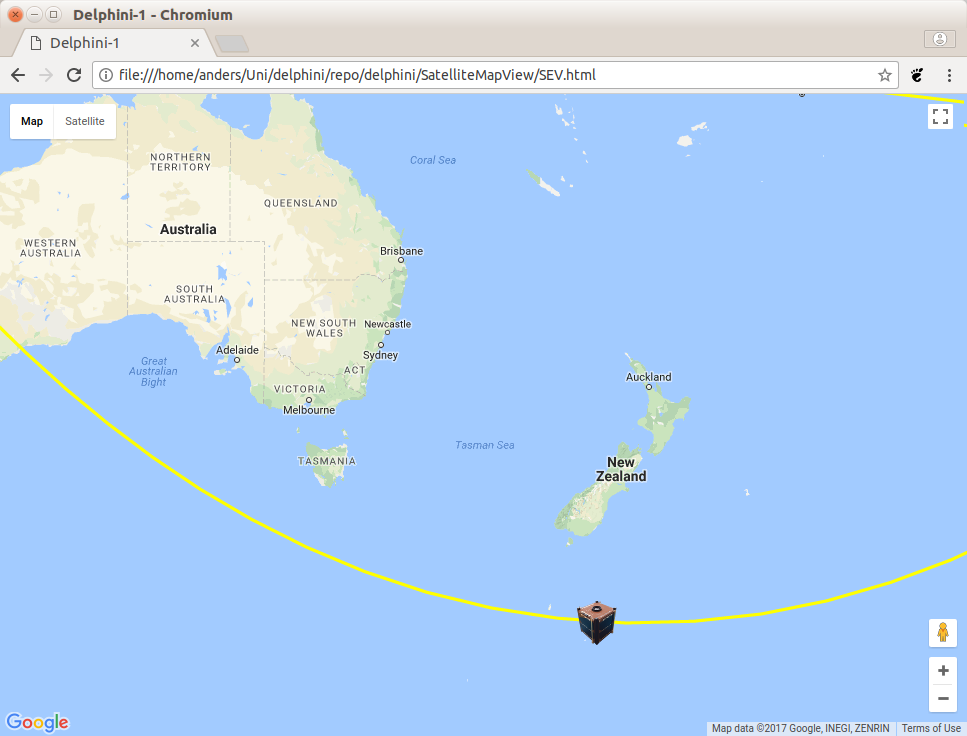
\includegraphics[width=\textwidth]{../SMV.png}
\caption{\texttt{SMV} showing a live updating map of ISS's position and orbit.}
\label{Fig:SMV}
\end{figure}

\subsection{Satellite Earth View}
\texttt{SEV} shows a satellite-tracking view of Earth, see Fig. \ref{Fig:SEV}. The application is powered by Google Earth Pro, a free mapping software available on Windows, Mac and Linux. Google Earth has support for a wide range of custom made input, such as graphical overlays, animated tours, etc. This input is created in the Keyhole Markup Language (KML), which is a format based on the Extensible Markup Language (XML). KML is the official standard recognized by the Open Geospatial Consortium. I have developed a simple Python routine that will create a KML file containing a track of the satellite's coordinates (specified by latitude, longitude and altitude) as a function of time. The Python routine uses a two-line element set as input and simply computes coordinates from a chosen start date to an end date. By opening the KML file in Google Earth, it is possible to play back the track. It is possible to display a view from satellite's position at any time (past, current or future). Note that \texttt{SEV} does not take into account any information about the camera (e.g. field of view, resolution, etc.). It simply presents a view of Earth from a given set of (latitude, longitude, altitude). The camera angle, playback speed, etc. is customizable. Google Earth has support for displaying a daily updated cloud cover map and accurate day/night lighting.

\subsection{Satellite Map View}
\texttt{SMV} displays the satellite's current position, live updating, on a interactive 2D map, see Fig. \ref{Fig:SMV}. The front end of \texttt{SMV} is written in HTML and JavaScript (using the Google Maps Javascript API) and will run in any modern webbrowser. The back end is powered by \texttt{sattrack}. In addition to showing the satellite's current position, it is possible to plot map overlays in the KML format. Examples include showing the orbit, a marker indicating the ground station, markers showing positions of scheduled images, etc. These overlays can be constructed either directly from KML files or using the graphical interface of Google My Maps (\texttt{google.com/mymaps}). 



\section{User Manual}
The routines are hosted at \texttt{github.com/ajustesen/delphini}. The Python routines are written for Python 2.7 and requires the modules \texttt{numpy} and \texttt{ephem}. The routines have been tested with the latest version of these modules on Ubuntu 16.04. The instructions (and this report) are also contained in the README file in the repository.

\subsection{Instructions for Satellite Earth View}
-- Download and install \href{https://earth.google.com/download-earth.html}{Google Earth Pro}.\\
-- Under \texttt{Tools -> Options -> Touring}, use the following settings:\\
%
\begin{figure}[H]
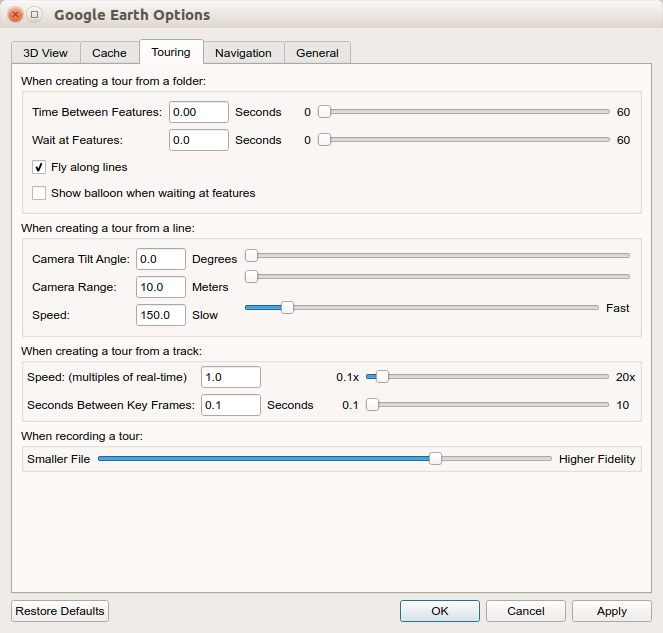
\includegraphics[width=1.0\textwidth]{../GoogleEarthSettings.png}
\end{figure}
%
\noindent -- Create a KML file using the Python script \texttt{create\_KML\_file.py} (instructions inside) and open it with Google Earth.\\
-- Make sure that Google Earth is set to UTC time in the \texttt{Date and Time Options} by clicking the icon highlighted in red below:\\
%
\begin{figure}[H]
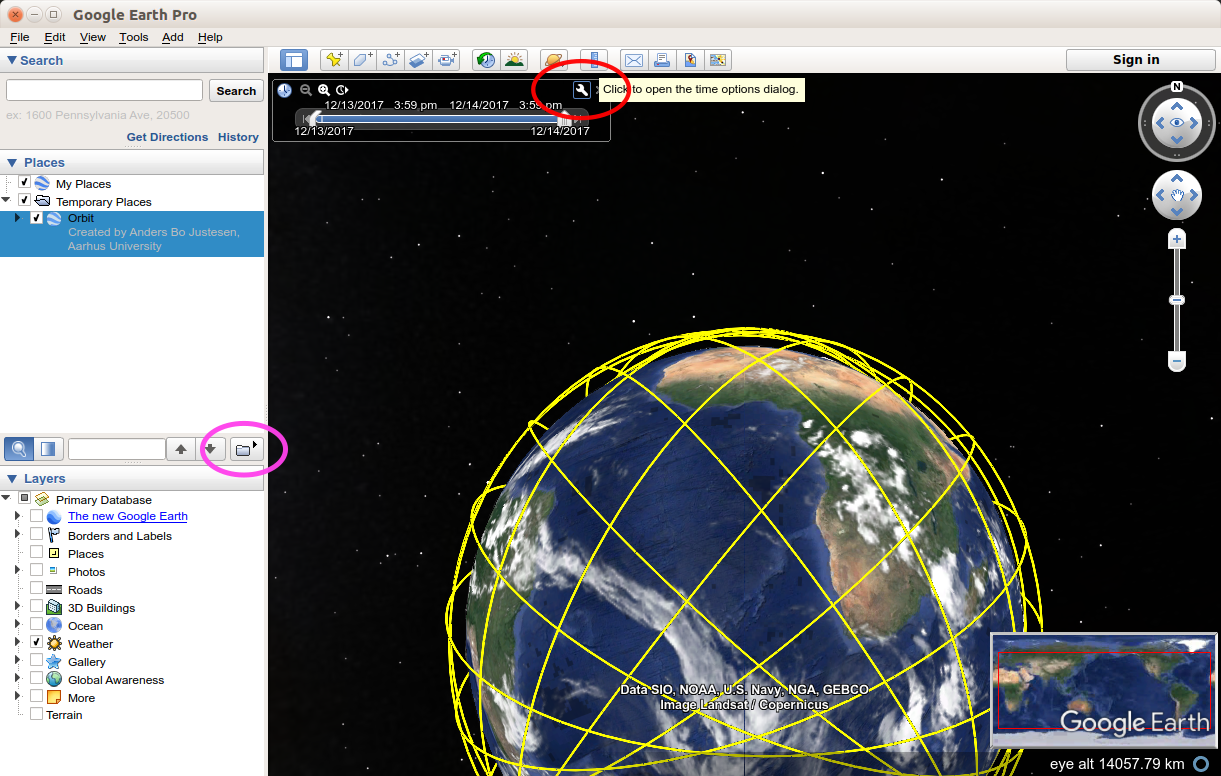
\includegraphics[width=1.0\textwidth]{../DateTime_PlayTour.png}
\end{figure}
%
\noindent -- To start \texttt{SEV}, press the \texttt{Play Tour} button highlighted above in pink.\\

\noindent \texttt{SEV} will start playing from the \texttt{startdate} you set in the \texttt{create\_KML\_file.py} script. To sync \texttt{SEV} to a realtime view, simply navigate to the current date and time. You can toggle layers (such as day/night view, cloud map, etc.) in the side bar under \texttt{Layers}.

\subsubsection{Instructions for Satellite Map View}
The executable Python script \texttt{compute\_coordinates} must be running in a terminal. When \texttt{compute\_coordinates} is active, it will update the coordinates every 250ms and save them to a file \texttt{coord.js}.\\
-- Make sure that \texttt{compute\_coordinates} has execute permission (\texttt{chmod +x compute\_coordinates}).\\
-- Start \texttt{compute\_coordinates} with a TLE file in the terminal, e.g.:
\begin{align*}
\texttt{./compute\_coordinates ISS.TLE}
\end{align*}
Optionally use the \texttt{--verbose} flag to display coordinates in the terminal. If you want to change the KML overlay (to plot e.g. the orbit), simply change the \texttt{url} to your favorite KML file in \texttt{SMV.html} at this point in the code (the default KML layer shows the ground station but not the orbit):
\begin{verbatim}
/* Load KML layer from URL or local path */
new google.maps.KmlLayer({
  map: map,
  url: 'https://www.google.com/maps/d/kml?mid=1919HD6uTNVHiKjLJFXtOXJqB00cuDFEe',
  preserveViewport: true
});
\end{verbatim}
\noindent -- With \texttt{compute\_coordinates} running, simply open \texttt{SEV.html} in a web browser.
\end{document}